\chapter{Simulation}

%--------------------------------------------------------------------------------------------------------
% 		Intro
%--------------------------------------------------------------------------------------------------------
\section{Intro}

In this section, we create realistic scenarios that model the environments of some of its applications.  
For example, the random movement of a mobile phone user around source nodes or a car moving at varying speeds around source nodes.  
By examining the performance evaluations of the message ferrying design using parametric studies., it can predict how it will perform in its environment and applications.
Furthermore, these parameters will enable the upd
These varied parameters are explained in section \ref{sec:metrics}.

%More realistic scenario
%	- Random ferry movement
%		- Details -> car
%	- even source spacing

%--------------------------------------------------------------------------------------------------------
% 		Topology
%--------------------------------------------------------------------------------------------------------
\section{Network Model}

In Figure \ref{fig:scenario2}, our scenario for the packet .  
The size of this topology is 1km x 1km.  
That is the distance between source node 0 and 4 is 1km, while the distance between source node 6 and 2 is also 1km.  
The speed of the ferries is random and the direction is random, where the speed is within 36kph to 72kph in a uniform distribution.  



%Might not need subsections for Scenario 1 & 2

\subsection{Scenario 1}

%1 gw, 1 ferry
This scenario has one gateway and one ferry node.
The parameters will be collected from the results.

%overview of the scenario2 (1f1g random movement)
\begin{figure}[h]
    \centering
    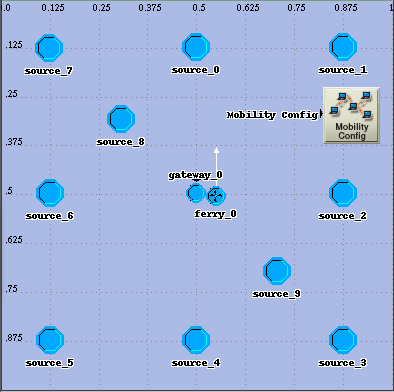
\includegraphics[width=.5\textwidth]{images/scenario2-top}
    \caption{Topology of Scenario 2}
    \label{fig:scenario2}
\end{figure}


\subsection{Scenario 2}

%2 gw, 2 ferry

%overview of the scenario3 (2f2g random movement)
\begin{figure}[h]
    \centering
    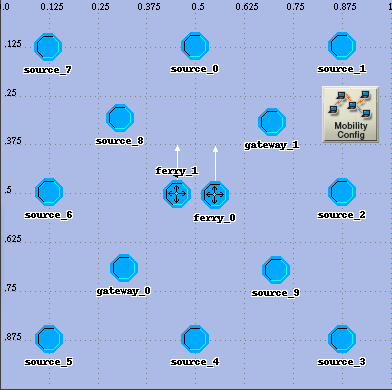
\includegraphics[width=.5\textwidth]{images/scenario3-top}
    \caption{Topology of Scenario 3}
    \label{fig:scenario3}
\end{figure}


\subsection{Common Settings}

%Characteristics of random ferry movement
%	- Speed 
%	- Beaconing intervals
%	- Property update interval


%--------------------------------------------------------------------------------------------------------
% 		Metrics and Results of Interest 
%--------------------------------------------------------------------------------------------------------
\section{Metrics and Results of Interest }
\label{sec:metrics}

%Some introduction

\subsection{Success Rate and Loss}
%Result of Interest 1: Success rate
%	- Main parameter of interest affecting success rate -> memory size
%	- Need to talk about what constitutes success rate

\subsection{Delay}
%Result of Interest 2: Delay
%	- Main parameter of interest affecting delay -> number of ferries & gateways
%	
%Something about delay for lost packets

\subsection{Parameters Varied} %TODO: better section title

The following factors have been considered when designing scenarios:
One of the parameters is to measure a so-called packet loss, by varying the buffer size limit.
Because of the nature of the algorithm, there may be dropped packets when the update number is older.
This packet loss is defined as where it measures the number of packets dropped when the buffer is full, and the oldest packets are dropped to accommodate for adding the new packet.  
We define our packet loss as the number of packets dropped due to the fact that the buffer size limit has been reached.
The other parameter is to measure the delay which is defined by the time to update the central repository once the update packet is sent out.

\subsubsection{Memory Limit}
In the following graph, we can see that the buffer size used is proportional to the rate of successful packets delivered to ferries.
%graph of results for buffer size vs. packet loss [uncomment this when ready]
%\begin{figure}[h]
%    \centering
%    \includegraphics[width=.5\textwidth]{images/result1}
%    \caption{Buffer size versus packet drop rate }
%    \label{fig:result2}
%\end{figure}
As seen from Figure \ref{fig:result2}, as the buffer size increases the packet loss decreases.
The red curve indicates the buffer size of ,......

\subsubsection{Number of Ferries and Gateways}
%See topology section
%gateway scenario
The increase of the number of gateways reduced the delay of updating to central repository.  
This result was expected because we knew that by properly placing another gateway in the area will grant better coverage.  
\subsection{Seed - Effect of Randomness}

\subsection{Source Node Storage}
